\documentclass[../../spr.tex]{subfiles}

\begin{document}

\section{Testy}
\subsection{Opis metod testowania (np. testy manualne i automatyczne)}
W projekcie zastosowano kombinację testów manualnych i automatycznych w celu zapewnienia jakości oprogramowania. Testy automatyczne skupiają się na komponentach interfejsu użytkownika, sprawdzając ich zachowanie w różnych scenariuszach. Testy manualne wykorzystano do weryfikacji ogólnej funkcjonalności systemu oraz integracji między modułami.

\subsection{Wyniki testów, napotkane błędy oraz zastosowane rozwiązania}

Przeprowadzone testy objęły wszystkie karty wykorzystywane w interfejsie użytkownika. Weryfikowano m.in. poprawność renderowania pól z określonymi wartościami, wywołania funkcji po wysłaniu formularza oraz widoczność elementów generowanych warunkowo.

Do testowania wykorzystano framework \textit{Vitest} oraz tryb przeglądarkowy, umożliwiający podgląd na żywo przebiegu testów. Próby użycia trybu \textit{headless} (bez interfejsu graficznego) skutkowały fałszywymi błędami, wynikającymi m.in. z braku interakcji z oknem (np. kliknięcia) lub problemów z~mockowaniem natywnych funkcji przeglądarki, ponieważ testy w tym trybie uruchamiane są w środowisku \textit{Node.js}. Wprowadzenie testowania w trybie przeglądarkowym wyeliminowało te problemy.

Podczas testów nie stwierdzono błędów w działaniu interfejsu – wszystkie kluczowe funkcjonalności działały zgodnie z oczekiwaniami. Jedyną napotkaną trudnością było połączenie interfejsu z~API, co wymagało refaktoryzacji nazw atrybutów komponentów oraz ich dostosowania do przypadków, w których dane mogą nie zostać pobrane. 

Znaczącym wyzwaniem okazała się również obsługa autoryzacji. Konieczne było utworzenie kontekstu użytkownika zintegrowanego z danymi pobieranymi z serwisu \textit{Keycloak} oraz implementacja \textit{interceptora} dla biblioteki \textit{axios}, umożliwiającego prawidłowe odświeżanie sesji użytkownika. Dodatkowo potrzebny okazał się komponent odpowiedzialny za kontrolę dostępu do chronionych ścieżek i przekierowywanie niezalogowanych użytkowników. Ostatecznie proces logowania został pomyślnie wdrożony i działa poprawnie.

\begin{figure}[H]
  \centering
  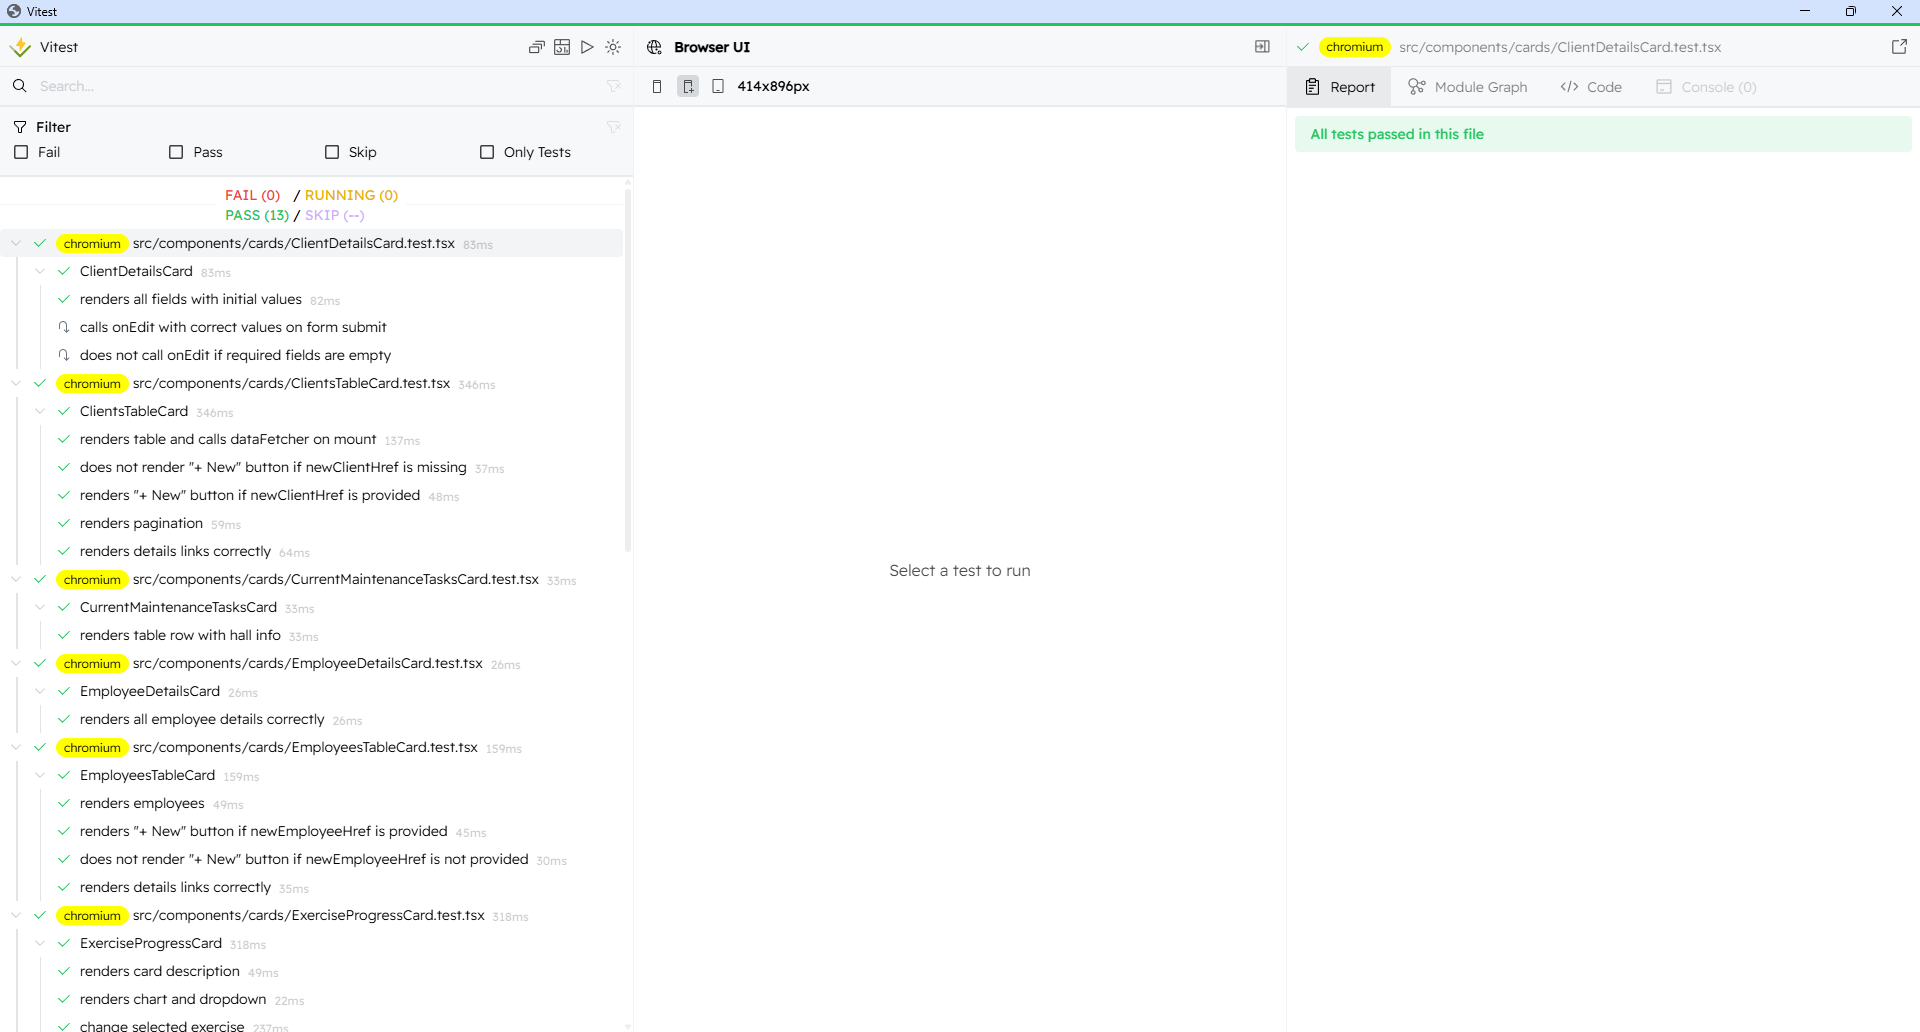
\includegraphics[width=\textwidth]{img/test.png}
  \caption{Wyniki testów interfejsu w środowisku \textit{Vitest}.}
\end{figure}

\end{document}